\chapter{Fejlesztői dokumentáció} % Developer guide
\label{ch:impl}

% ==========================================================
% |                Használt technológiák                   |
% ==========================================================
\section{Használt technológiák}
Az alkalmazás fejlesztését JavaScript nyelven kezdtem meg és fejlesztés közben váltottam TypeScript nyelvre. A TypeScript gyakorlatilag egy típusos kiterjesztése a JavaScriptnek, éppen ezért minden kód amit JavaScriptben írtam azok érvényes és valid kódok TypeScriptben is. A TypeScript lényege, hogy típus biztossá teszi az alkalmazást, ami ugyan megnehezíti a fejlesztést, de nagy előnye, hogy sok probléma már a fejlesztés során észlelhető - ezáltal javítható - és nem a kész verzióban történnek katasztrofális dolgok. Váltásom motivációja a TypeScript nyújtotta előnyök mellett az is volt, hogy az ipar jelenlegi trendjei teljesen egészében effelé a nyelv felé mutatnak, minden komolyan vehető program - amely Electront, Angulart vagy más hasonló webes technológiát használ - már TypeScript nyelven íródik. Ez predesztinálta az én hozzáállásomat is a nyelvhez, tekintve a legelejétől fogva célom volt a legfrissebb és legnépszerűbb technológiák haszálata, ezen piacképes tudások elsajátítása.

Az alkalmazás fejlesztése teljes egészében a Visual Studio Code nyílt forráskódú kódszerkesztővel zajlott, Electron-t, React-et és Redux-ot továbbá Git verziókezelő rendszert felhasználva és egy publikus GitHub repositoryban tárolva a kódot, amely elérhető az alábbi címen: \url{https://github.com/TMD44/mvp}

\subsection{Electron}
Az Electron\footnote{\url{https://www.electronjs.org/}} egy nyílt forráskódú keretrendszer, amelyet asztali alkalmazások fejlesztéséhez lett kifejlesztve. Különlegessége, hogy a már ismert és bejáratott webes technolgiákat - tehát HTML, CSS, JavaScript - lehet használni asztali alkalmazások fejlesztéséhez. Az Electron két külön, egymástól hermetikusan elzárt része a {\it main process} és a {\it renderer process}, melyek között alá-fölé rendelt viszony található.

Az Electron ``fő szála'' - ezt nem véletlenül tettem idézőjelbe, tekintve a JavaScript egy egyszálú programozási nyelv, tehát JavaScriptben nem tudunk konkurrens programokat írni -, vagy hívhatjuk angolul {\it main process}nek is, ami gyakorlatiag egy Node.JS alkalmazás, amely a böngésző ablakok létrehozásáért, az operációs rendszerrel való kommunikációért és az alkalmazás életciklusárt felel. Ez gyakorlatilag egy fájl, amely az alkalmazásunk belépési pontját fogja képezni.

Az előbb említett böngésző ablak pedig az Electron másik elszeparált és alárendelt része, a {\it renderer process}, amelyet a {\it main process} hoz létre és menedzseli is azt. Ez tulajdonképpen egy Chromium böngésző ablakot fog jelenteni, amely egy HTML fájlt fog megjeleníteni, ahogy azt a webes világban már megszokhattuk. Lehetőgésünk van továbbá Node intergrációhoz is, amit a {\it main process}en belül tudunk engedélyezni. Az integráció lényege, hogy a böngésző ablakból használhatjuk a Node által nyújtott funckiókat is, például fájlrendszer elérése, modulok importálása és exportálása.

\subsection{React}
A React\footnote{\url{https://reactjs.org/}} egy JavaScript könyvtár, amely főleg felhasználó felületek készítésére nyújt egy fölöttébb elegáns megoldást. A segítségével rendkívül egyszerűen tudunk, úgy nevezett Single Page Application-ket készíteni. Az innováció ebben a megközelításben az, hogy nincs szükség az oldal újbóli betöltésére, hanem a felhasználói interakció során az oldal tartalmai dinamikusan újratölthetőek és nem is az egész oldal, hanem annak kisseb részei, úgy nevezett komponensei.

\subsection{Redux}
A Redux\footnote{\url{https://redux.js.org/}} egy state management tool, vagyis magyarul egy állapot kezelő rendszer. A Redux lényege és legnagyobb előnye, hogy az alkalmazásunk állapotát képes külön, egy külön egységként tárolni és menedzselni. Az állapotot memóriában tárolja, gyakorlatilag egy nagy JSON objektumban, ezen adatok módosítása pedig {\it dispatch} útján valósítható meg.

% ==========================================================
% |                 Megvalósítási terv                     |
% ==========================================================
\section{Megvalósítási terv}

\subsection{Követelmény specifikáció}
Az alkalmazás működéshez és a feladatleírás teljesítéséhez az alábbi funkciókat kell implementálni:
\begin{itemize}
    \item {\textbf {Film felsoroló platform: }} Az alkalmazásnak felületet kell biztosítania a beolvasott média tartalmak megjelenítéséhez, listázásához.
    \item {\textbf {Média tartalmak beolvasása: }} Mappák kiválasztásával az azokban fellelhető média tartalmak beolvasása.
	\item {\textbf {Keresés a média tartalmak között: }} Az alkalmazásnak lehetőséget kell bizotsítania a beolvasott média tartlamak közötti kereséshez.
	\item {\textbf {Lejátszás, Megállítás, Pörgetés: }} Bizotsítania kell a videók lejátszását.
	\item {\textbf {Felirat választás: }} Feliratok megjelenítése lejátszáskor, amennyiben elérhető.
	\item {\textbf {Sorozatok és filmek kezelése: }} A felület kezelje külön a sorozatokat és filmeket, tehát például a sorozat epizódjai ne külön-külön jelenjenek meg a listában, hanem a sorozatra rákkatintva, annak részletező ablakjában legyenek listázva az epizódok.
	\item {\textbf {Metaadatok betöltése és letölése: }} Használható és értelmes adatok beolvasása fájlnévből, mappanévből, NFO fájlból és külső adatbázisból metadatokat kell tudnia letölteni.
    \item {\textbf {Lejátszási listák: }} Lehessen lejátszási listákat létrehozni, ezen listákat filmekkel feltölteni.
\end{itemize}

\subsection{Adatok tárolása, kezelése}
Az alkalmazás futása közben a Redux segítségével kezeljük a felhasznlói felülethez és a beolvasott média tartalmakhoz kapcsolódó adatokat. Reduxot főleg webalkalmazásokhoz használnak, de nekünk itt asztali környezetben is alkalmazható lesz egy kis trükkel, mégpedig amikor megnyitjuk az alkalmazást, a Redux beállítja a kezdeti állapotot - ez a webes körnezetben annyit tenne, hogy egy előre meghatározott alapértelmezett állapot sémát alakalmazna - ami a mi esetünkben két fájl lesz, a {\it config.json} és a {\it mediaDB.json}. A {\it config.json} fájl az alkalmazás futásához, a beolvasáshoz és a felhasználó személyes preferenciáihoz szükséges adatokat, míg a {\it mediaDB.json} a beolvasott média tartalmakhoz kapcsolodó adatokat, metaadatokat tartalmazza. Ez a két JSON fájl két féleképpen jöhet létre:
\begin{itemize}
    \item Létrejöhet az alkalmazás bezárásakor, ekkor az alkalmazás jelenlegi állapota kerül kiírásra a fájlba.
    \item Valamint létrejöhet az alkalmazás indításakor is, ha a program úgy érzékeli, hogy a megadott helyen még nem létezik ez a két fájl. Ilyenkor egy előre megadott alapértelmezett állapot kerül kiírásra, amely alapértelmezett beállításokat (felhasználói felület, beolvasásssal kapcsolatos preferenciák stb.) és egy üres vázat tartalmazza, amelybe bekerülnek majd a scannelés során gyűjtött adatok.
\end{itemize}

\begin{figure}[H]
	\centering
	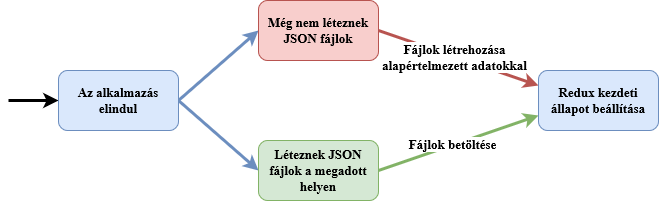
\includegraphics[width=1\textwidth]{Redux_init.png}
	\caption{A Redux kezdeti állapot beállítása}
	\label{fig:redux-init}
\end{figure}

Tehát az alkalmazás futása közben az adatok a Redux store-ban tárolódnak, amikor az alkalmazás bezárásra kerül, akkor az állapot két fájlba kerül kírásra - ebből fakadóan két futás között az adatok fájlban átrolódnak - amit aztán újranyitás esetén egyszerűen betöltünk a kezdeti állapotba.

\subsubsection{Példa config.json fájl}

\lstset{caption={Példa config.json fájl}, label=src:json}
\begin{lstlisting}[language={json}]
{
"creation_time": "2021.05.10. 12:00:00",
"modification_time": "2021.05.10. 12:00:00",
"user_info": { "name": "Anonymous" },
"app_info": {
    "app_name": "Multimedia Visualization Platform",
    "app_version": "0.1.0",
    "app_current_directory": "G:\\mvp\\src\\main",
    "app_locale": "hu",
    "app_locale_country_code": "HU",
    "app_paths": {
        "home": "C:\\Users\\tmd-pc",
        "user_data": "C:\\Users\\tmd-pc\\AppData\\Roaming\\Multimedia Visualization Platform",
        "desktop": "C:\\Users\\tmd-pc\\Desktop",
        "downloads": "C:\\Users\\tmd-pc\\Downloads",
    }
},
"scan_preferences": {
    "scan_language": "en-US",
    "scan_paths": [ "G:\\SOROZATOK" ],
    "scan_file_types": {
        "media": [ ".mkv",".mp4",".avi" ],
        "sub": [ ".srt",".ass",".vtt",".ssa",".sub",".stl",".scc" ],
        "nfo": [ ".nfo" ]
    },
    "scan_results": {
        "media": [{
            "fn": "Game.of.Thrones.S01E01.BDRIP.x264.Hun.Eng",
            "ext": ".mkv",
            "path": "G:\\SOROZATOK\\Game.of.Thrones.COMPLETE.BDRIP.x264.Hun.Eng",
            "full": "G:\\SOROZATOK\\Game.of.Thrones.COMPLETE.BDRIP.x264.Hun.Eng\\Game.of.Thrones.S01E01.BDRIP.x264.Hun.Eng.mkv"
            }],
        "sub": [{
            "fn": "Game.of.Thrones.S01E01.BDRIP.x264.Hun.Eng",
            "ext": ".srt",
            "path": "G:\\SOROZATOK\\Game.of.Thrones.COMPLETE.BDRIP.x264.Hun.Eng",
            "full": "G:\\SOROZATOK\\Game.of.Thrones.COMPLETE.BDRIP.x264.Hun.Eng\\Game.of.Thrones.S01E01.BDRIP.x264.Hun.Eng.srt"
            }],
        "nfo": [{
            "fn": "Game.of.Thrones.COMPLETE.BDRIP.x264.Hun.Eng",
            "ext": ".nfo",
            "path": "G:\\SOROZATOK\\Game.of.Thrones.COMPLETE.BDRIP.x264.Hun.Eng",
            "full": "G:\\SOROZATOK\\Game.of.Thrones.COMPLETE.BDRIP.x264.Hun.Eng\\Game.of.Thrones.COMPLETE.BDRIP.x264.Hun.Eng.nfo"
            }],
    }
}}
\end{lstlisting}

\subsubsection{Példa mediaDB.json fájl}

\lstset{caption={Példa mediaDB.json fájl}, label=src:json}
\begin{lstlisting}[language={json}]
{
"creation_time": "2021.05.09. 14:44:49",
"modification_time": "2021.05.09. 14:44:49",
"movies": {
    "23b5b6d765ac7a28badbd2f6e6d31ea3": {
        "id": [ "23b5b6d765ac7a28badbd2f6e6d31ea3" ],
        "media_type": "movie"
    },
    "6209ef3cb9451c0def78013521b84d5f": {
        "id": [ "6209ef3cb9451c0def78013521b84d5f" ],
        "media_type": "movie"
    },
},
"tv_series": {
    "Game of Thrones": {
        "id": [
            "98cddc3eb8b19c7ebb2a84049c5fc4f0",
            "6a216938ea15d2a1e5282ec47d9a0649",
            "6044b7976f57147dd35da9c3719fd921",
        ],
        "media_type": "series"
    }
},
"playlists": {
    "Game of Thrones Best of": {
        "contents": {
            "Game of Thrones": {
                "id": [
                    "98cddc3eb8b19c7ebb2a84049c5fc4f0",
                    "6a216938ea15d2a1e5282ec47d9a0649",
                    "6044b7976f57147dd35da9c3719fd921",
                ],
                "media_type": "series"
            }
        },
        "media_type": "playlist"
    }
},
"all_media": {
    "98cddc3eb8b19c7ebb2a84049c5fc4f0": {
        "id": "98cddc3eb8b19c7ebb2a84049c5fc4f0",
        "media_name": "Game.of.Thrones.S01E01.BDRIP.x264.Hun.Eng",
        "extension": ".mkv",
        "path": "G:\\SOROZATOK\\Game.of.Thrones.COMPLETE.BDRIP.x264.Hun.Eng",
        "full_path": "G:\\SOROZATOK\\Game.of.Thrones.COMPLETE.BDRIP.x264.Hun.Eng\\Game.of.Thrones.S01E01.BDRIP.x264.Hun.Eng.mkv",
        "subtitles": [ "G:\\SOROZATOK\\Game.of.Thrones.COMPLETE.BDRIP.x264.Hun.Eng\\Game.of.Thrones.S01E01.BDRIP.x264.Hun.Eng.vtt" ],
        "nfo": "G:\\SOROZATOK\\Game.of.Thrones.COMPLETE.BDRIP.x264.Hun.Eng\\Game.of.Thrones.COMPLETE.BDRIP.x264.Hun.Eng.nfo",
        "metadata": {
            "title": "Game of Thrones",
            "season": 1,
            "episode": 1,
            "languages": ["HUN", "ENG"],
            "codec": "X264",
            "quality": "BDRIP",
            "media_type": "series",
            "imdb_id": "tt0944947",
            "imdb_url": "https://www.imdb.com/title/tt0944947"
        }
    },
}}
\end{lstlisting}

\subsection{Média tartalmak beolvasása}
Az alkalmazás egyértelműen legfontosabb része a média tartalmak beolvasása. Ezt három részre lehet lebontani
TODO

\subsubsection{Mappa kiválasztás}
A mappák megnyitásához az Electron egy beépített modulját, a ``dialog''ot fogjuk használni. A probléma csak az, hogy ezt a modult nem leszhet a renderer processben használni csak a main processben, ilyenkor jön jól az IPC renderer és IPC main modulok amelyek kommunikációt tesznek lehetővé a két réteg között. Az ``Open Dir'' gombra kattintva tehát elküldjük az IPC-n keresztül a main process-nek, ami aztán a ``dialog'' modult felhasználva megnyitnya az operációs rendszer natív párbeszédablakját, ebben az esetben kifejezetten mappák megnyitását engedélyezzük csak, azokból is többet. Az ablakot bezárva az eredményt string tömb formájában visszaküljük a renderer processnek, amely elvégzi a Redux store-ba dispatch-elését. A config objecten belül ``scan paths'' kulcs néven találjuk a beolvasott mappák tömbjét.

\lstset{caption={Mappák megnyitása}, label=src:python}
\begin{lstlisting}[language={python}]
ipcMainCommunication.on('open-dir-sync', (event) => {
    dialog
        .showOpenDialog(window, {
            properties: ['openDirectory', 'multiSelections'],
        })
        .then((result) => {
            if (result.canceled === false) {
                event.returnValue = result.filePaths;
            } else {
                event.returnValue = [];
            }
        })
        .catch((err) => {
            console.log(err);
        });
});
\end{lstlisting}

\subsubsection{Offline scan}
Az Offline scannelés megkezdéséhez két dologra lesz szükségünk, az egyik a mappák amelyekben keresni fogunk, a másik hogy milyen fájl típusokat fogunk keresni, igencsak hatékonytalan lenne ha minden fájlt beolvasnánk amelyek a program működését tekintve nem lényeges információkat tartalmaznak, éppen ezért szűrni fogjuk a fájlokat. A Redux store-ból tehát behívjuk a ``scan file types'' kulcshoz tartozó objektumot amely egy tematikusan tömböket tartalmazó objektum, ezek előre meghatározott fájltípusok, a felhasználónak lehetősége van megváltoztatni őket. Behívjuk továbbá az előző pontban hozzáadott ``scan paths''-eket.

A megadott mappa elérési utvonalakon végig iterálva minden útvonalra meghívjuk a ``scanDir'' függvényt amely rekurzívan a mappa tartalmán - amennyiben a mappában még több mappa található, ezekben az estekben is hasonlóképpen jár el - és a megadott fájltípusokra szűrve egy tömbbe pusholja a talált fájlokat (videófájlok, például ``.mkv'',``.mp4'' vagy felirat fájlok, például ``.srt'', ``.vtt'', illetve NFO fájlok ``.nfo''). Történik még egy filterezé ezt követően, tekintve nagyon sok példa van rá, hogy az offline videó tartalmaink mellet úgy nevezett ``sample'' vagy minta videó fájlok is helyt kapnak, ezek a fájlok szűrésre kerülnek, ugyanis a program működésének szempontjából lényegtelen fájlokról beszélünk. Eztuán minden talált elemet átalakít egy sokkal kezelhetőbb formátumra, a fentebb már config.json példában bemutatott ``scan\_results'' kulcsban. A lényeg itt annyi, hogy a megfelelő formátumú fájlokat a megfelelelő objektumbra szortírozzuk, tehát média fájlokat a media objektumba, a felirat fájlokat a sub objektumba, az NFO fájlokat pedig az nfo objektumba. Mindezek elvégzése után elmentjük a Redux store-ba megintcsak dispatch útján.

\lstset{caption={Mappák megnyitása}, label=src:python}
\begin{lstlisting}[language={python}]
const { media, sub, nfo } = getScanFileTypes();
const paths = getScanPaths();

for (const i in paths) {
    const files = await scanDir(paths[i], [media, sub, nfo].flat());
    for (const j in files) {
        if (!excludedFromScan(files[j])) {
            fileSorting(files[j], media, sub, nfo, scanResults);
        }
    }
}
store.dispatch(addScanResults(scanResults));
const results = getScanResults();

for (const file in results.media) {
    const result = await mediaJSONGenerator( results.media[file], results );
    scan.mediaInJSON[result.id] = result;
}
store.dispatch(addMediaAtOnce(scan.mediaInJSON));
\end{lstlisting}

A következő for ciklusban már ezeket az átalakított objektumokat fogjuk felhasználni és tovább alakítjuk ``mediaJsonGenerator'' függvény segítségével. A függvény elször összepárosítja a felirat fájlokat a hozzá kapcsolódó videófájlhoz, tekintve a feliratfájloknál eddig is az volt a konvenció, hogy a felirat fájl neve legyen ugyanaz mint a videó fájl neve, ezt felhasználva könnyű dolgunk van. Végeredményben egy tömböt fogunk kapni, amely tartalmazza a videó fájlhoz köthető feliratokat. A felirat fájlokkal történik a program ezen pontján még egy fontos dolog, mégpedig egy ``.vtt'' formátumra konvertálás, ennek oka az, hogy habár asztali alkalmazást készítünk az eszköztár amelyet használunk webes technológiákra épülnek éppen ezért igazodnunk kell a web által támogatott formátumokra, amely jelen esetünkben felirat fájlok esetén a ``.vtt''.

Eztuán az NFO fájl - általában egy NFO fájl köthető egy videó fájlhoz - videófájlhoz párosítása következik. Ez már kicsit bonyolultabb eset, itt is fenn áll ugyan a ``legyen ugyanaz a neve'', de a fájlstruktúrán belül a fájl elhelyezkedése változhat. Sorozatok esetén például általában nincs mindegyik epizódhoz külön NFO fájl, hanem magához az évadhoz vagy az egész sorozathoz, tehát a fájl helye nem feltétlenül a videó fájl mellet található. A scannelés folyamata lekezelei ezeket a különböző eseteket, tehát végeredményben megkapjuk a videófájlhoz köthető NFO fájlt.
Innentől kezdve rendelkezünk tehát NFO fájllal amely rengeteg hasznos offline információt tartalmaz a filmünkről, azonban itt olyan problémába ütközünk, hogy az NFO fájl tartalmát tekintve semmilyen konvenció vagy szokás nincs, éppen ezért algoritmikus úton kifejezetten nehéz biztosan helyen információkat kinyerni. Ennek következtében az NFO fájlban kifejezetten csak a legfontosabb információt fogjuk keresni, mégpedig egy IMDB linket. Az IMDB a legelterjedtebb filmes adatbázisok egyike jelenleg és az url címében a film egy egyedi azonosítója található, amelyet fel fogunk tudni használni majd a metaadatok letöltésekor. Az NFO fájl tartalmának beolvasását követően, egy reguláris kifejezés segítségével ({\it /tt[0-9]{7,8}/gi}) IMDB azonosítót keresünk, ha találtunk akkor nincs is más dolgunk mint lementeni egy objektumba, amit aztán visszaadunk a ``mediaJsonGenerator'' függvénynek. Abban az esetben ha nem találtunk explicit azonosítót, megpróbálkozunk megképp.
Számos esetben megfigyelhető, hogy az NFO fájlokban URL rövidítő szolgáltasokat használnak, például TinyURL, Bit.ly stb. Scannelésünk folyamatában rendkívül fontos információ az IMDB ID, éppen ezért az algoritumus az egyik legnépszerűbb a TinyURL visszafejtésével is megpróbálkozik. Abban az esetben ha sikerrel jár és a rezolválás eredménye egy IMDB azonosító akkor a már fentebb ismeretett módon járunk el, ha nem járunk sikerrel akkor az információ nem kerül bele az eredmény objektumba.

A másik forrás amelyből offline használható információkat tudunk kinyerni, a fájlnév és a mappa neve. Ehhez a fájl név felismerő függvényünket fogjuk használni, amely az NFO-s azonosító felismeréshez hasonlóan regulásris kifejezések szövegre illesztésével fogjuk kivitelezni.
Az ``fnr'' függvény a következő képpen működik, megkap egy stringet, ami az egyik esteben a fájl neve, a másik esetben a mappa neve. Ezután ezután sorban, reguláris kifejezéseket illeszt a szövegre és ha illeszkedik rá azt a szövegből kivesszük és a visszaadandó eredmény objektumba rakjuk, az eredeti stringben pedig aláhúzás (\_) karakterre cseréljük a talált eredményt. Ezt minden egyes Regex típusra eljátszuk, ennek következtében a végére kapunk egy eredmény objektumot amelyben tematikusan szét van válogatva a talált stringek, illetve a visszamaradó stringet amelyben már csak a cím maradt az egyetlen hasznos információ. Ekkor az algoritmus a string elejétől elkezd ``értelmes karaktereket'' keresni tehát kisbetűs, nagybetűs karakterek illetve számok, és addig megy a szövegben amíg el nem kezd találni minimum kettő vagy annál több ``értelmetlen kataktereket'', ezek az aláhúzás (\_), a pont (.) és a szóköz ( ). Ha 2 vagy több értelm ``értelmetlen kataktert'' találtunk, akkor az addig ``értelmes'' karaktereket kimentjük, ez lesz a cím. Továbbá kicsit szépítünk is rajta például ha a szavak között pont van azt szóközre cseréljük és az első karaktert nagybetűsre cseréljük. Abban az esetben ha valami hiba történik a cím keresésekor a string már üres, vagy rossz formátumú tehát üres stringet adna vissza, az algoritmus az eredeti, még a függvény paraméterül megkapott stringet teszi meg címnek.

\lstset{caption={Példa reguláris kifejezésekre}, label=src:python}
\begin{lstlisting}[language={python}]
const fnrPatterns = {
    resolution: /[0-9]{3,4}[PI]{1}|[0-9]{3,4}[.\-_ ]?[X][.\-_ ]?[0-9]{3,4}/gi,
    year: /((?:19[3-9]|20[0123])[0-9])/g,
    languages: /[.\-_ ](ENG|HUN|GER|JAP)[^a-zA-z]/gi,
    bluray: /BD[0-9]{2}|BD100/gi,
    season: /[.,\-_ ]S([0-9]{1,2})-(S)?([0-9]{1,2})|[.,\-_ ]S([0-9]{1,2})|[^0-9]([0-9]{1,2})X/gi,
    episode: /[.,\-_ ]E([0-9]{1,3})-(E)?([0-9]{1,3})|E([0-9]{1,3})(?:[^0-9]|$)|[Xx]([0-9]{1,3})(?:[^0-9]|$)|(EP|EPISODE)([0-9]{1,3})(?:[^0-9]|$)/gi,
    codec: /XVID|DIVX|AVC|HEVC|X[.\-_ ]?26[0-9]|H[.\-_ ]?26[0-9]/gi,
    audio: /(DD|DDP|MA|AC3|AAC|PCM|LPCM|FLAC|DTS[._\- ]?(HD)?|TRUEHD[+._\- ]?ATMOS|TRUEHD|ATMOS)[+._\- ]?[0-9]\.?[0-9]|DTS[._\- ]?(HD|ES)?|DUAL[._\- ]?AUDIO|DOLBY[+._\- ]?(DIGITAL[+._\- ]?(PLUS)?|VISION|ATMOS)|HALF-OU/gi,
};
\end{lstlisting}

Végeredményben tehát két objektumot fogunk visszakapni a függvénytől, egyet a fájlnévből kinyert adatokkal és egy másikat a mappa nevéből kinyert adatokkal, ezek egyesítése a következő függvény a ``dataSum'' feladata. Az alap logikánk egyszerű, éppen ezért kivitelezésünk is: az adatok egyesítése során azaz objektum lesz a domináns amelyik több kulcsot tartalmaz, a több kulcs több kinyert információt is jelent. Az eredmény objektumunkba először a kevesebb kulcsú objektumot rakjuk bele aztán ráengedjük a több kulcsú objektumot, ilyenkor kulcs egyezés esetén a másodjára jövő objektum felülírja a már meglévő kulcsot, ezáltal az eredmény objektumban benne lesz mind a két objektum egyedi kulcsai (amik csak a fájlnév objektumban és mappanév objektumban voltak), hasonló kulcsok esetén pedig a domináns, tehát több kulcsú objektum adatai maradnak meg. Ezáltal megkapjuk a metaadatok objektumot.

\lstset{caption={Példa az fnr függvény eredményére és egyesítésére}, label=src:python}
\begin{lstlisting}[language={python}]
FNR
\end{lstlisting}

Legvégül minden fent kiszűrt adatot összesítünk egy nagy objektumban, amely tehát tartalmazni fogja külön kulcsokra szétszedve a videó fájl nevét, kiterjesztését, elérési útvonalát, a felirat fájlok útvonalait (több is lehet), az NFO fájl útvonalát (egy lehet), a metaadatok objektumát, illetve egy egyedi ID azonosítót amelyet MD5-ös hasheléssel hozunk létre a videó fájl útvonalából, ez az azonosító az operációs rendszer által bizosítottan egyedi lesz, hiszen nem lehet 2 ugyanolyan nevű és kiterjesztésű fájl ugyanazon az útvonalon. Az eredményt pedig dispatcheljük a Redux storeba.

Az Offline scannelésből egy dolog maradt még hátra. Érdemes meggondolni ezen média tartalmak megjelenítését, az egy részet filmek megjelenítésével nincsen probléma, tekintve ezek egy videó fájlból állnak tehát egy ilyen média objektummal le tudjuk írni az összes hozzá köthető adatot. A probléma a többrészes sorozatoknál kezdődik ahol is több videó fájl található tehát több média objektum is. Éppen ezért megjelenítésnél nem az ``all\_media'' kulcson tárolt nagy objektumokat fogjuk megjeleníteni, hanem készítünk egy ``movies'' és egy ``tv\_series'' objektumot amelybe értelem szerűen a filmek és sorozatok kerülnek majd külön. Mindkét objektumba a média tartalmak ID azonosítóit fogjuk tenni, értelemszerűen filmek esetén egy egy azonosítót fog jelenteni, sorozatok esetében pedig midegyik epizód azonosítója bekerül. Az objektumok struktúrája mindkét esetben hasonló, hogy a megjelenítési feldoglozásnál ne kelljen külön lekezelni a két esetet. A 3.2-es forráskódban példát is hozunk minden fentebb leírtakra.

\subsubsection{Online scan}
Az Online scannelés keretein belül a The Movie Database\footnote{\url{https://www.themoviedb.org/}} (továbbiakban TMDB) API-ját fogjuk használni, amely egy szabadon, ingyenesen felhasználható interfészt biztosít a számunkra, továbbá az API egy Node-os impelentációját fogjuk még használni a ``node-themoviedb'' modult\footnote{\url{https://www.npmjs.com/package/node-themoviedb}}.

Az algoritmus végig iterál a összes beolvasott tartalmon és amennyiben talál IMDB azonosítót - fentebb már részleteztük, hogy mennyire fontos ez, hiszen így biztosan helyes információkat fogunk visszakapni - akkor az azonosító alapján megejti a kérési a TMDB API felé, amely helyes válaszküldés esetén, némi kissebb adatátalakítás - például az API-ból a műfajok szám azonosító formában jönnek vissza ezeket szövegeket tartalmazó tömbökké alakítjuk át - és kulcs átnevezés után bedispatcheljük a Redux storeban a metaadatok objektumba. A dispatchelés során ha egyező kulcsokat talál akkor a régi érték felülíródik az új értékkel, amennyiben pedig nincs egyezés úgy egyszerűen belekerülnek az objektumba.

Amennyiben nem talál IMDB azonosítót, de talált évszámot és címet, akkor ezek elapján intéz kérést az API felé, helyes viszontválasz esetén pedig a már fentebb leírtak hajtódnak véghez ebben az esetben is, tehát kissebb adatátalakítás után a Redux storba illesztés történik.

Miután ezzel ekészült szintén lefut média típus szétválogatás mint az Offline scannelés végén, tehát a filmek azonosítói a ``movies'' objektumba másoldonak bele, a sorozatok epizdójainak azonosítói pedid egy a ``tv\_series'' objektumon belüli tömmbe másolódnak bele.

\subsection{Felhasználói felület terve}
A felhasználói felület teljes mértékben React segítségével készült. Az alkalmazás felhasználói felületének belépési pontja az {\it index.html} és {\it index.tsx} fájl, amelyben a React render függvénye kerül meghívsára az App komponensen. Az App komponensen belül pedig a Layout komponensre megyünk tovább ahol a fő UI logika található.
Az felhasználói felületnek két fő megjelenítési felülete lehet, az egyik az úgy nevezett Main, ami a fő ablak tartalmát hivatott leírni és változtatni, a másik pedig a Modal, amely a fő ablakon belüli, alárendelt, belső ablakot nyit meg.
TODO

\begin{figure}[H]
	\centering
	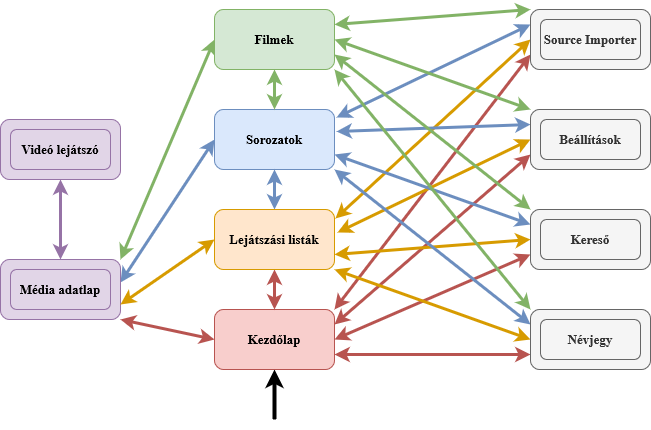
\includegraphics[width=1\textwidth]{navigation_between_screens.png}
	\caption{Navigáció az oldalak között}
	\label{fig:navigation_between_screens}
\end{figure}

\cleardoublepage
\subsection{Használati esetek diagram}
\begin{figure}[H]
	\centering
	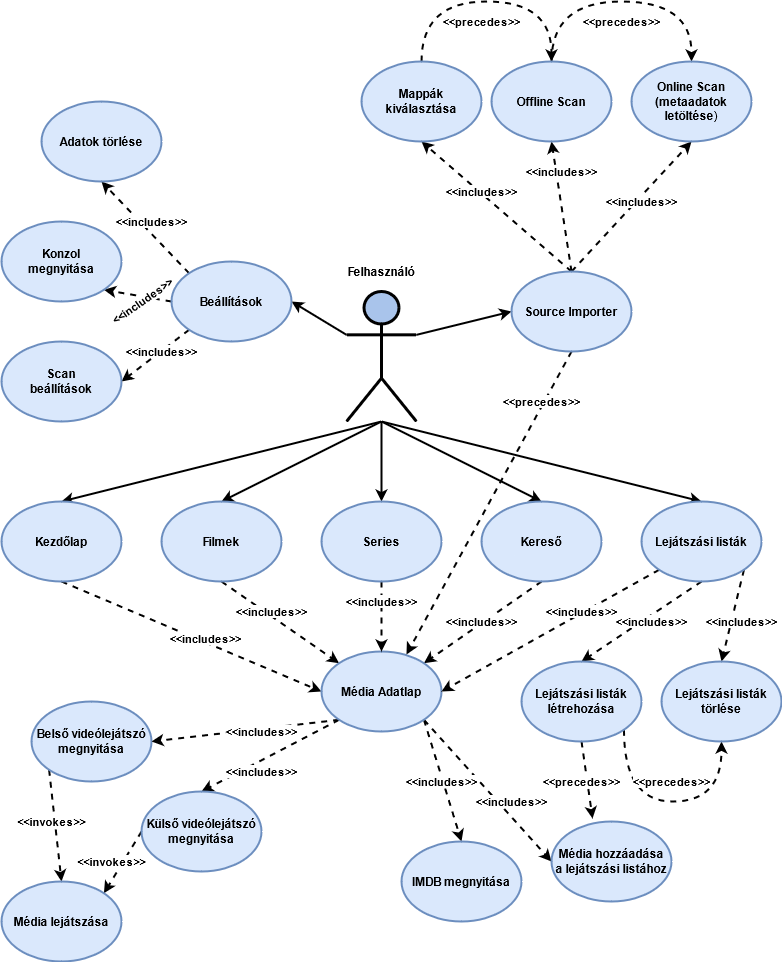
\includegraphics[width=1\textwidth]{use_case_diagram.png}
	\caption{Használati esetek diagram}
	\label{fig:use_case_diagram}
\end{figure}
\cleardoublepage

% ==========================================================
% |                    Implementáció                       |
% ==========================================================
\section{Implementáció}
TODO

\subsection{Funkcionális megközelítés}
TODO

% ==========================================================
% |                      Tesztelés                         |
% ==========================================================
\section{Tesztelés}
A fejlesztés a legelejétől kezdve gyakorlatilag folyamatos kézi tesztelés mellett zajlott.

\subsection{Hibás vagy eredménytelen megközelítések}
